\chapter{内嵌AA-CAES的灵活风机性能灵敏度分析}
\label{cha:ca-wt-para-sensitivity}

\section{几类典型的灵活风机参数}
\begin{figure}[H] % use float package if you want it here
  \centering
  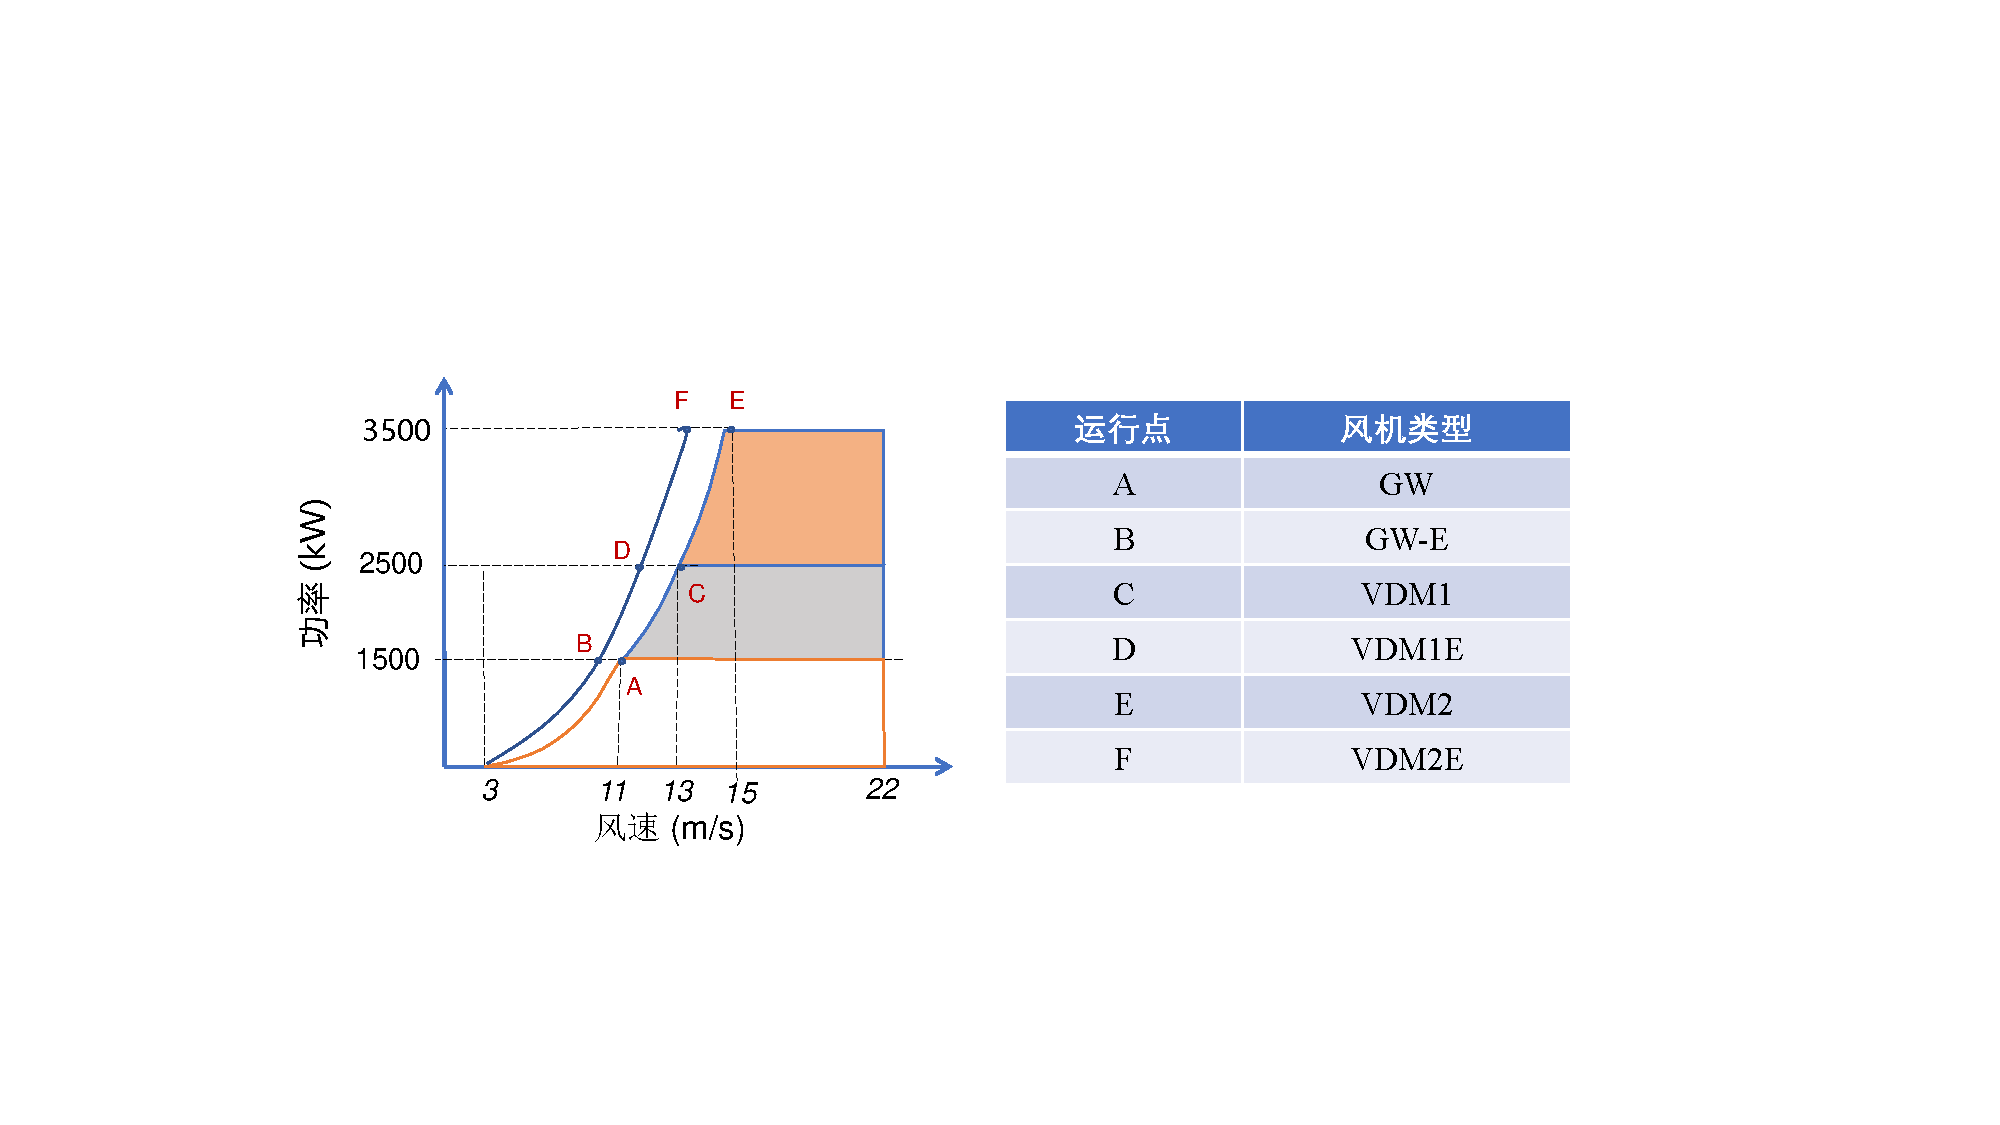
\includegraphics[scale=0.55]{figures/Chap5-CA-WT-Category.pdf}
  \caption{典型的传统风机及内嵌AA-CAES的灵活风机(额定电功率1.5MW)}
  \label{fig:CA-WT-Category}
\end{figure}

\section{风机性能及灵敏度分析}
\begin{figure}[H] % use float package if you want it here
  \centering
  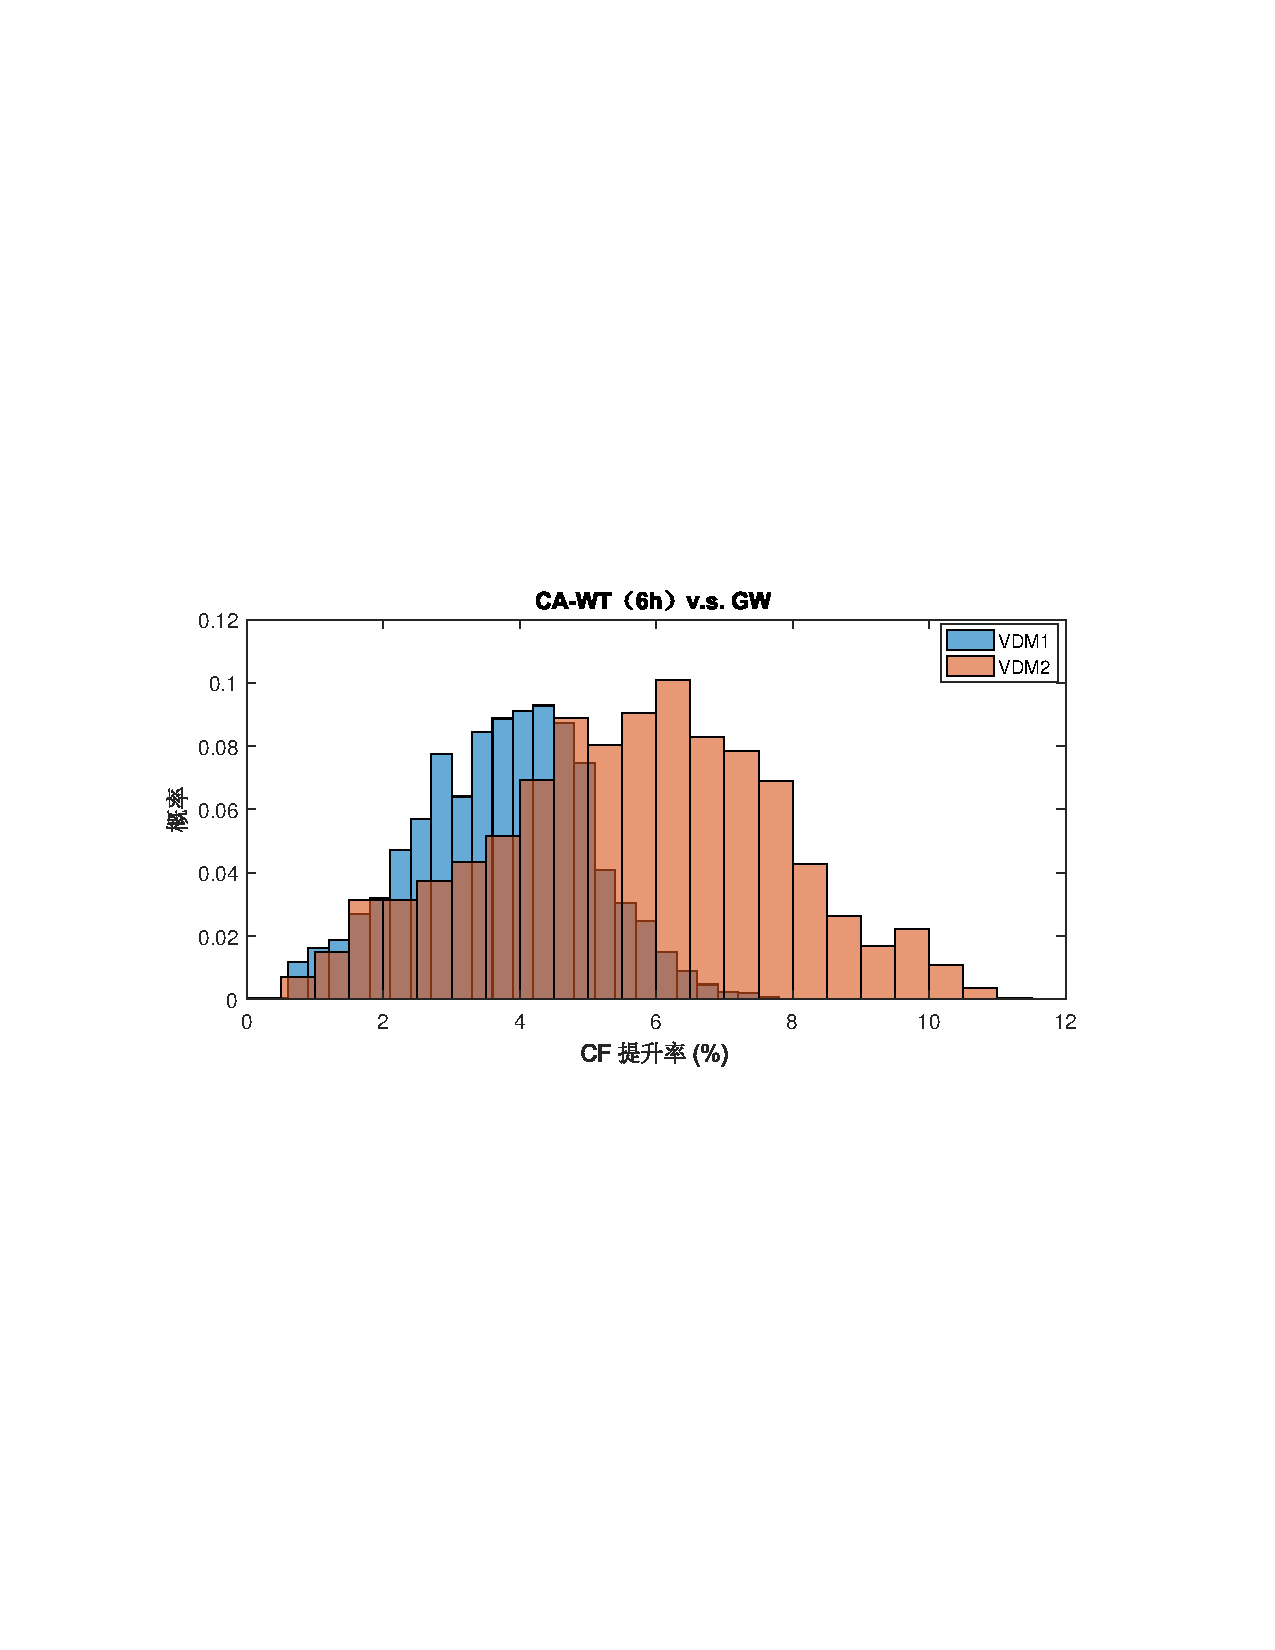
\includegraphics[scale=0.75]{figures/Chap5-CA-WT-6h-VS-GW-China.pdf}
  \caption{6h储能容量下压缩/膨胀机性能对比}
  \label{fig:CA-WT-6h-VS-GW-China}
\end{figure}

\begin{figure}[H] % use float package if you want it here
  \centering
  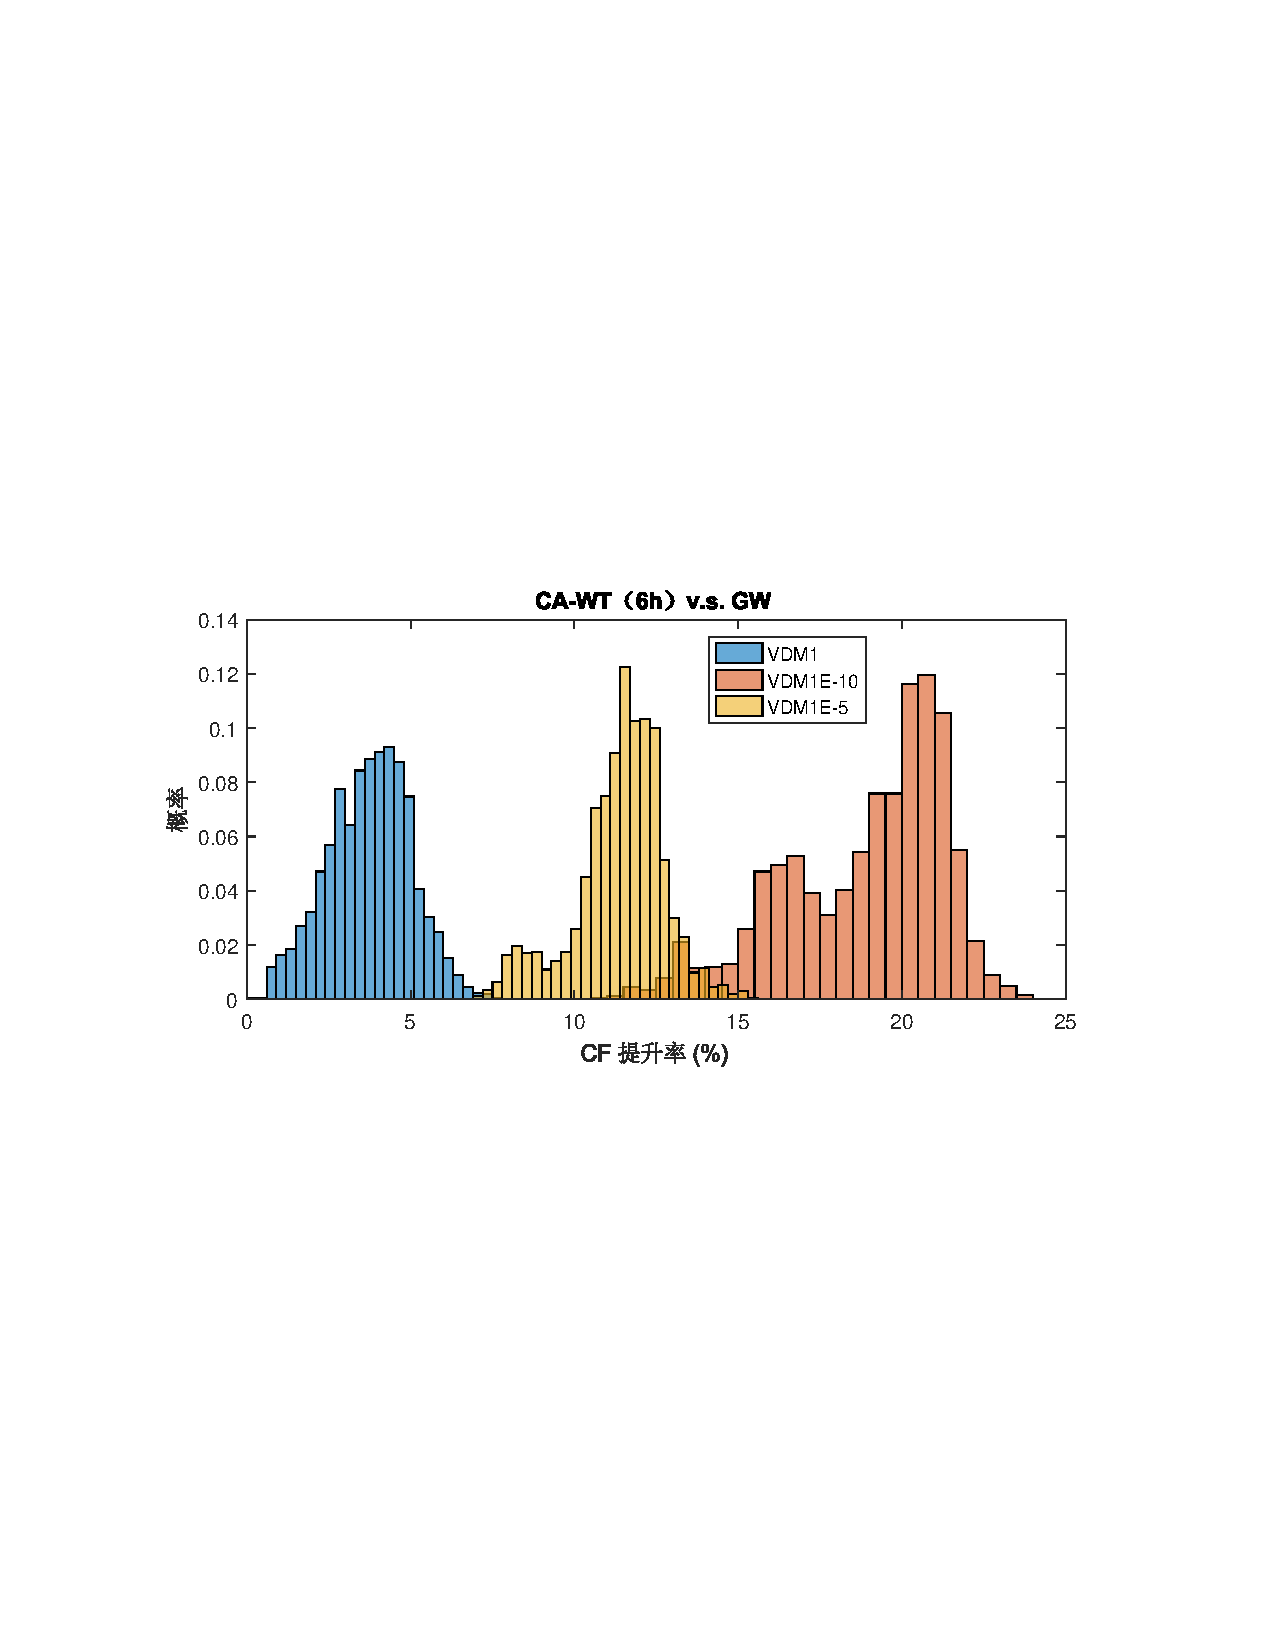
\includegraphics[scale=0.75]{figures/Chap5-CA-WT-6h-VS-GW-VDM1E.pdf}
  \caption{6h储能容量及VDM1方案下不同叶片尺寸性能对比}
  \label{fig:CA-WT-6h-VS-GW-VDM1E}
\end{figure}

\begin{figure}[H] % use float package if you want it here
  \centering
  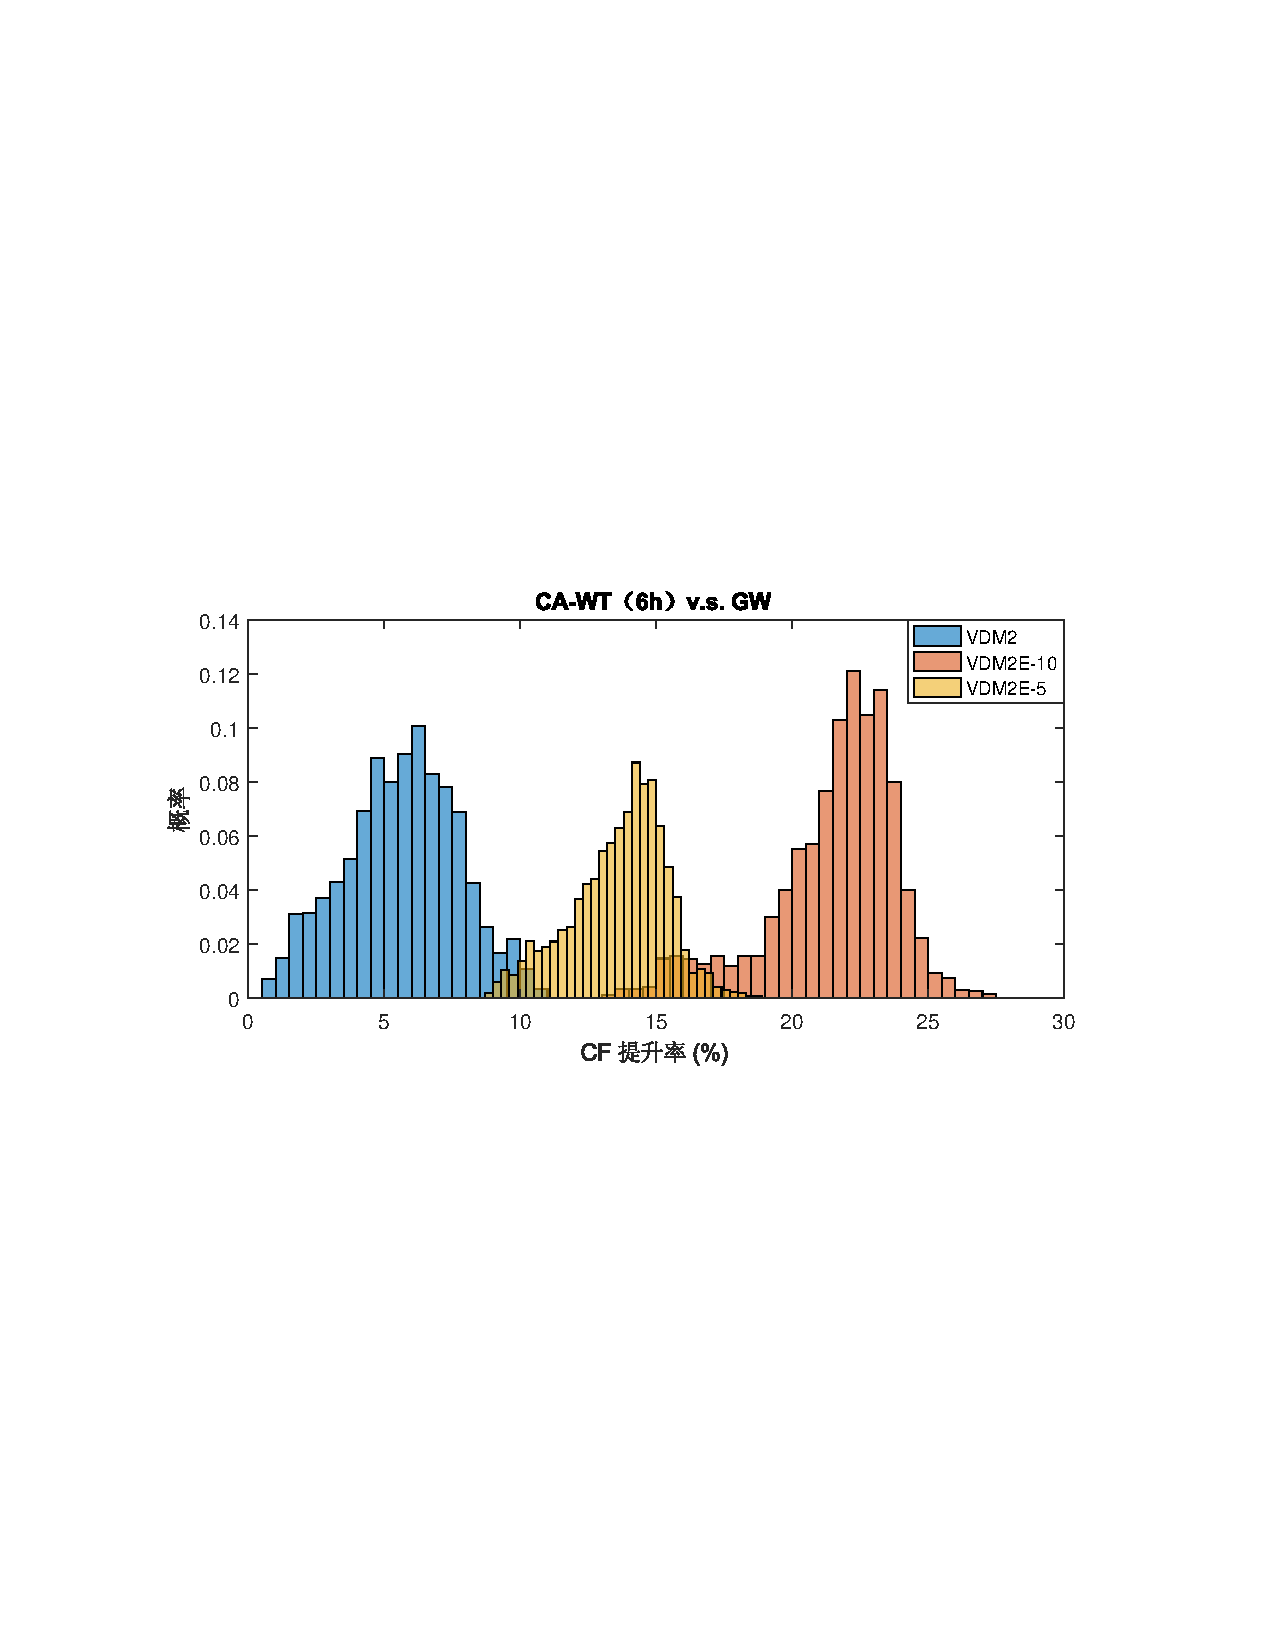
\includegraphics[scale=0.75]{figures/Chap5-CA-WT-6h-VS-GW-VDM2E.pdf}
  \caption{6h储能容量及VDM2方案下不同叶片尺寸性能对比}
  \label{fig:CA-WT-6h-VS-GW-VDM2E}
\end{figure}

\begin{figure}[H] % use float package if you want it here
  \centering
  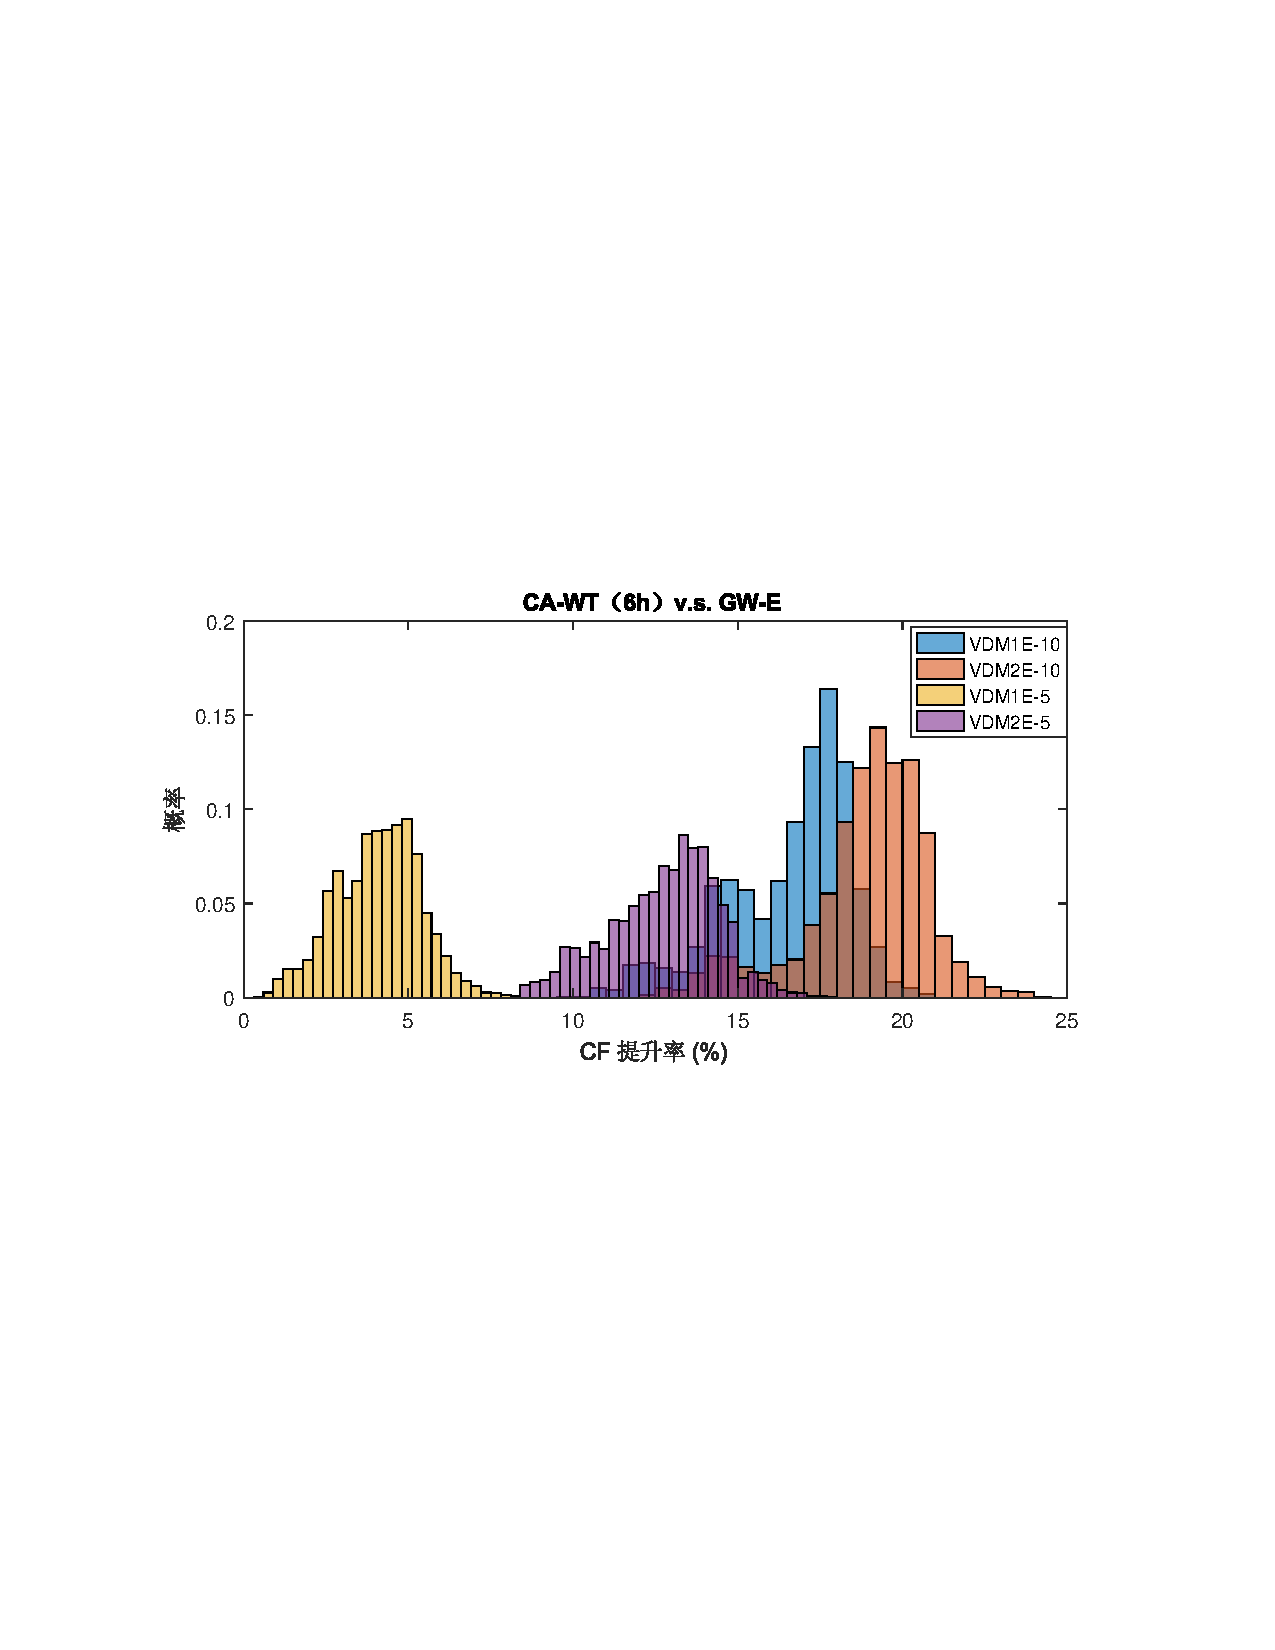
\includegraphics[scale=0.75]{figures/Chap5-CA-WT-6h-VS-GW-E.pdf}
  \caption{6h储能容量下叶片尺寸扩展的传统风机与灵活风机风机性能对比}
  \label{fig:CA-WT-6h-VS-GW-E}
\end{figure}

\begin{figure}[H] % use float package if you want it here
  \centering
  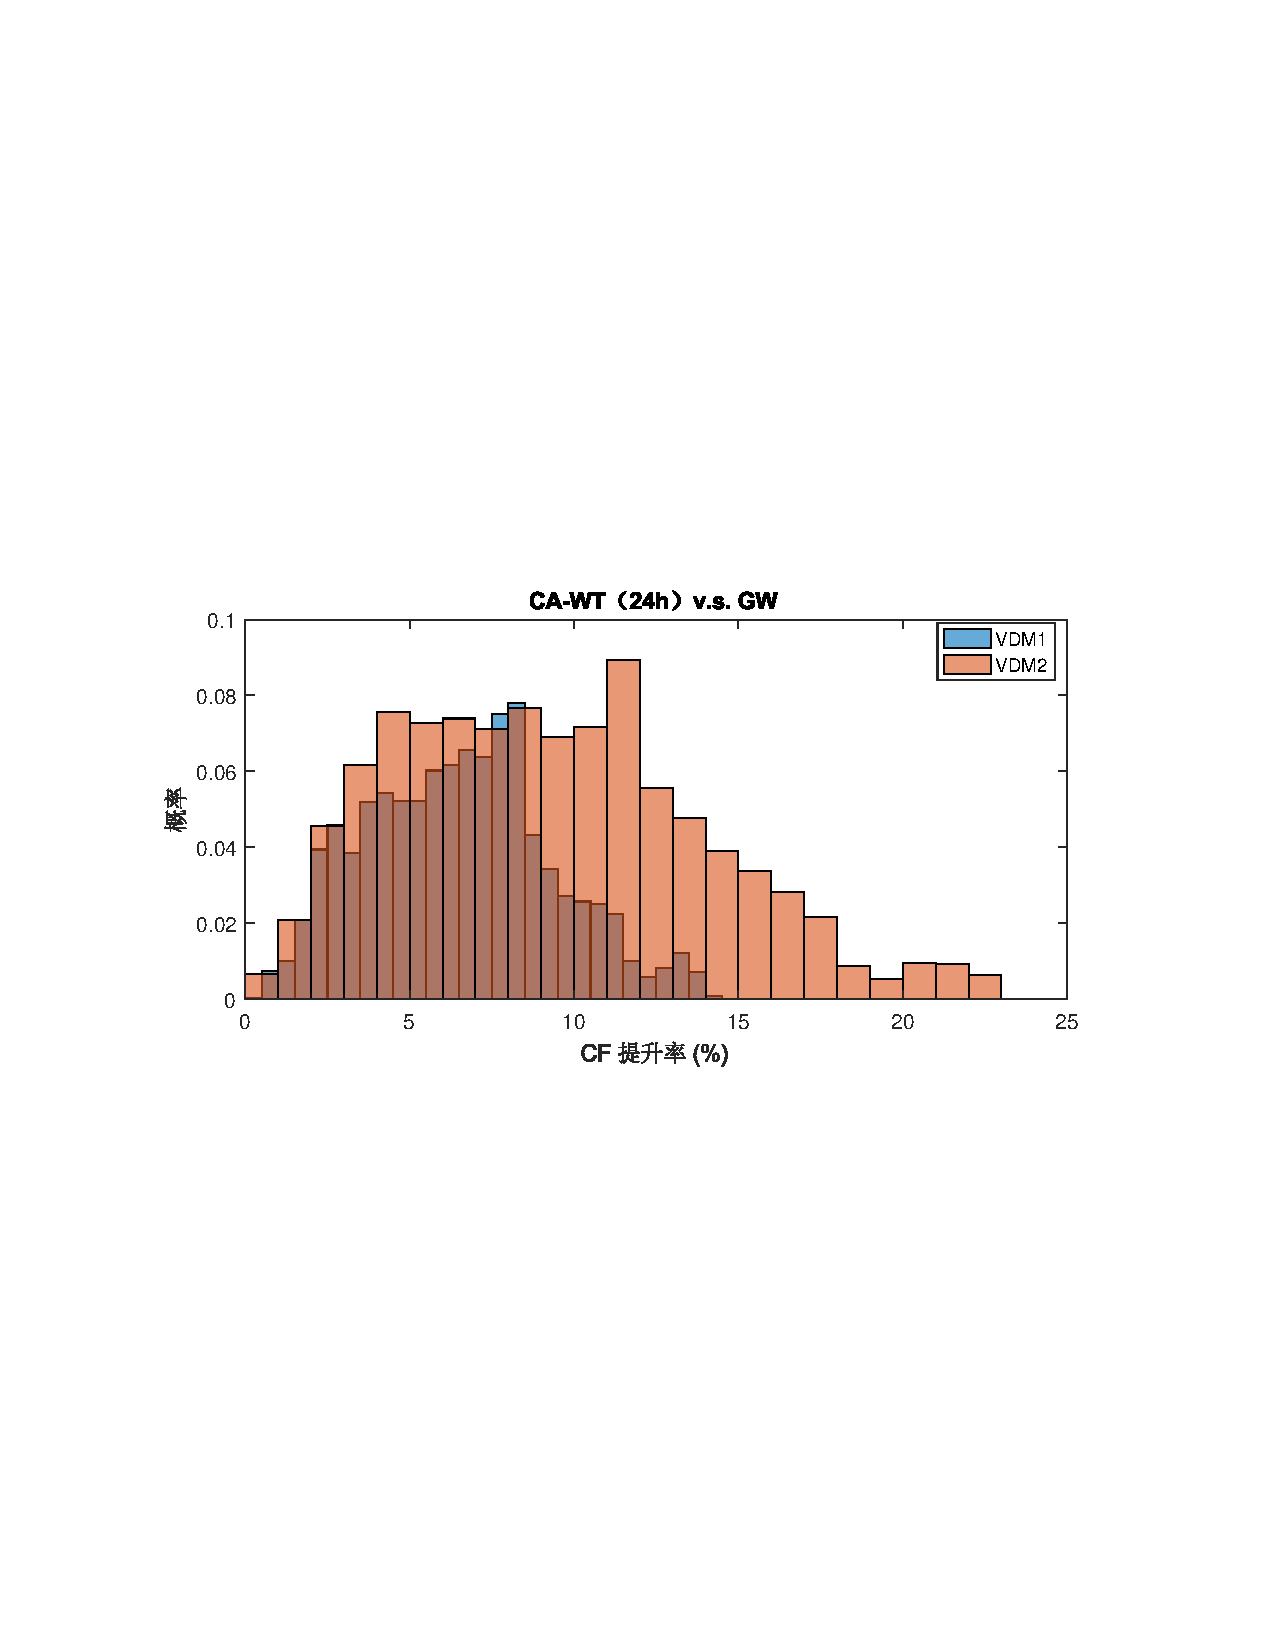
\includegraphics[scale=0.75]{figures/Chap5-CA-WT-24h-VS-GW-China.pdf}
  \caption{24h储能容量下压缩/膨胀机性能对比}
  \label{fig:CA-WT-24h-VS-GW-China}
\end{figure}

\begin{figure}[H] % use float package if you want it here
  \centering
  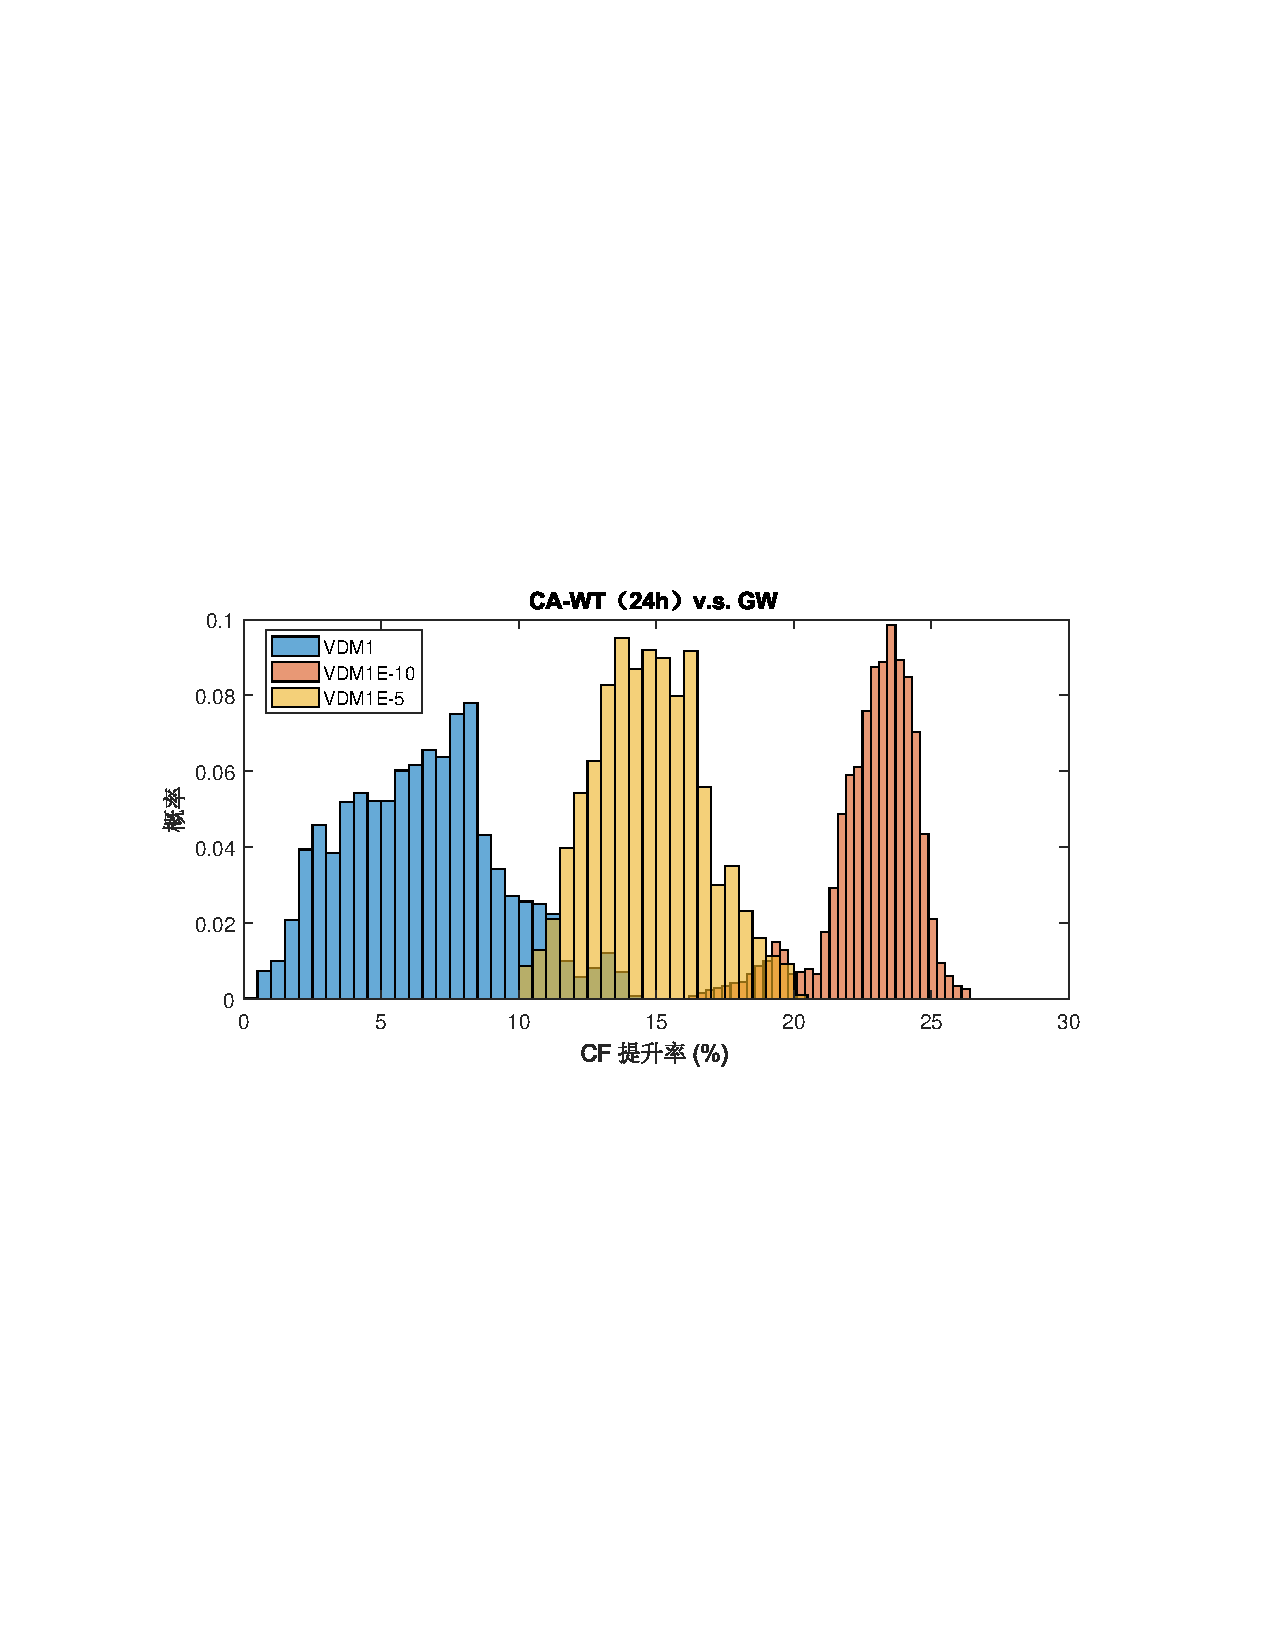
\includegraphics[scale=0.75]{figures/Chap5-CA-WT-24h-VS-GW-VDM1E.pdf}
  \caption{24h储能容量及VDM1方案下不同叶片尺寸性能对比}
  \label{fig:CA-WT-24h-VS-GW-VDM1E}
\end{figure}

\begin{figure}[H] % use float package if you want it here
  \centering
  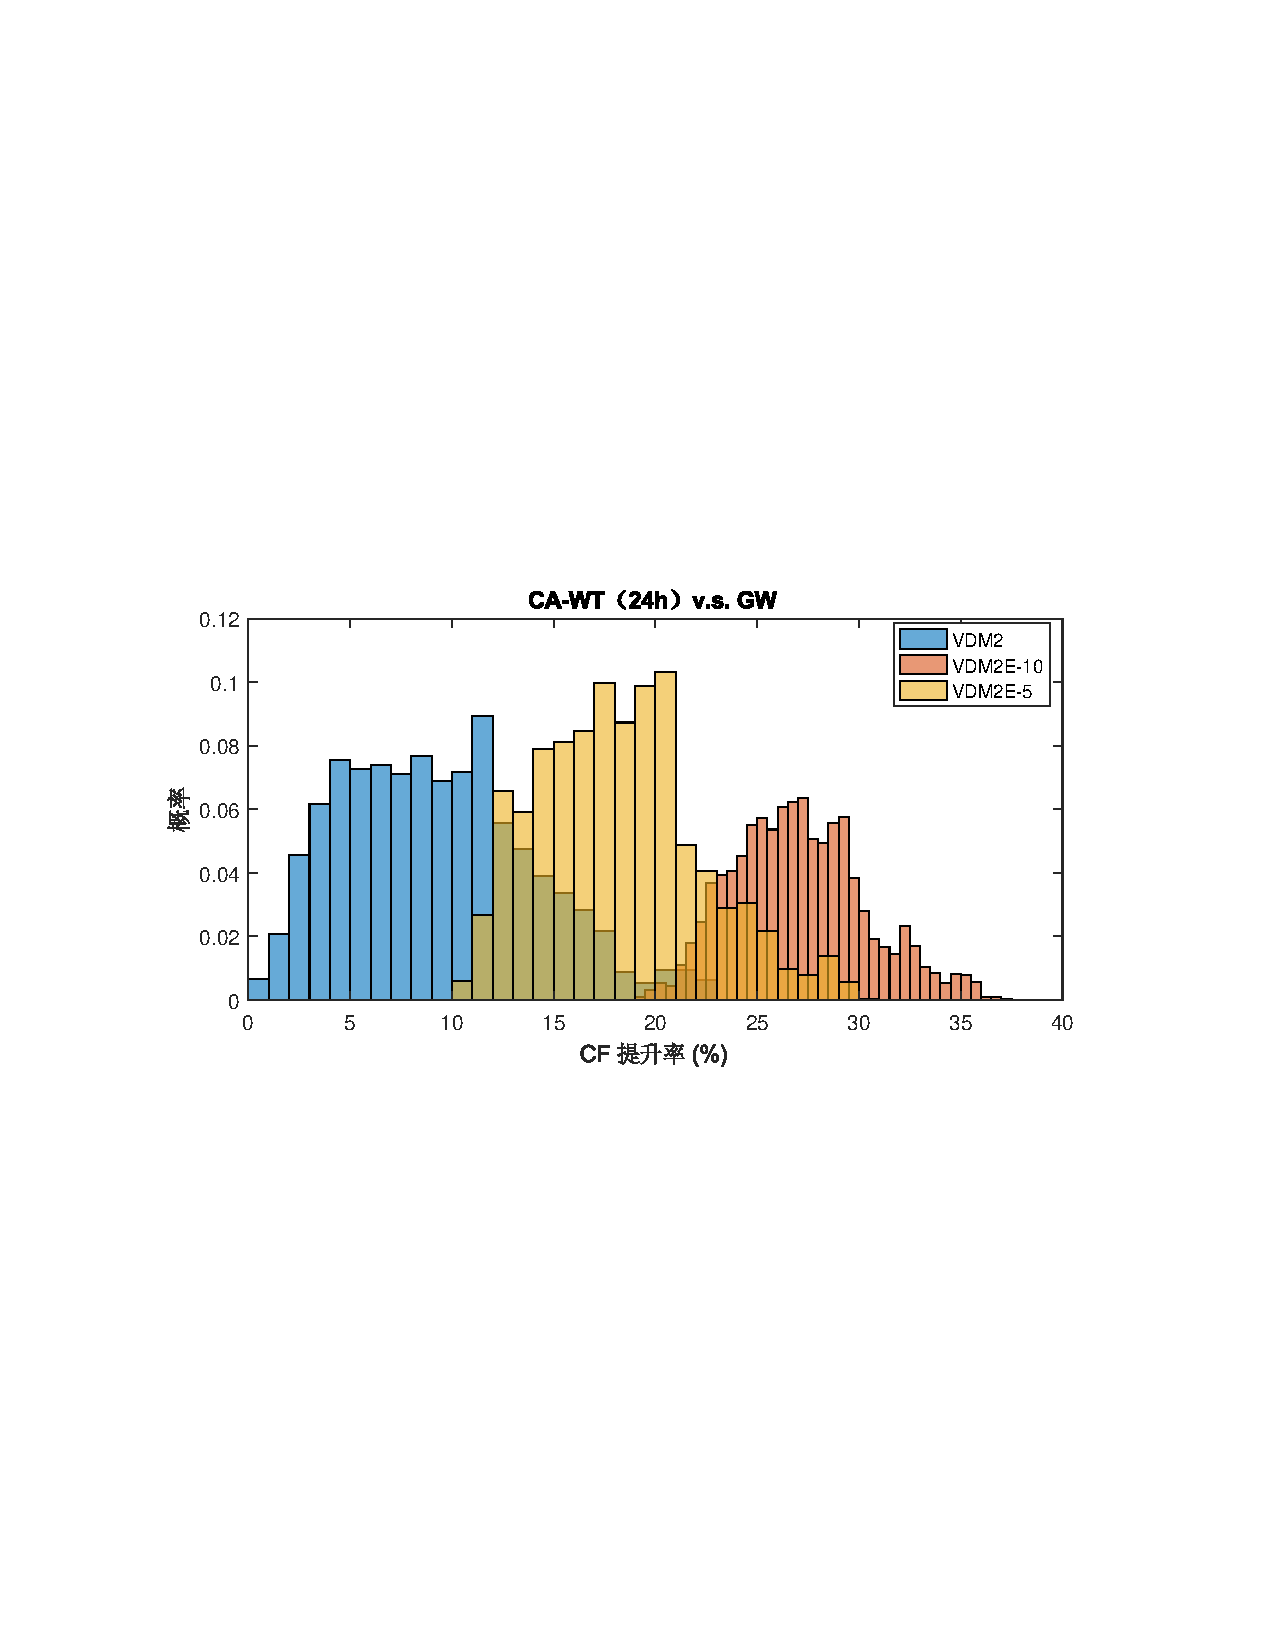
\includegraphics[scale=0.75]{figures/Chap5-CA-WT-24h-VS-GW-VDM2E.pdf}
  \caption{24h储能容量及VDM2方案下不同叶片尺寸性能对比}
  \label{fig:CA-WT-24h-VS-GW-VDM2E}
\end{figure}

\begin{figure}[H] % use float package if you want it here
  \centering
  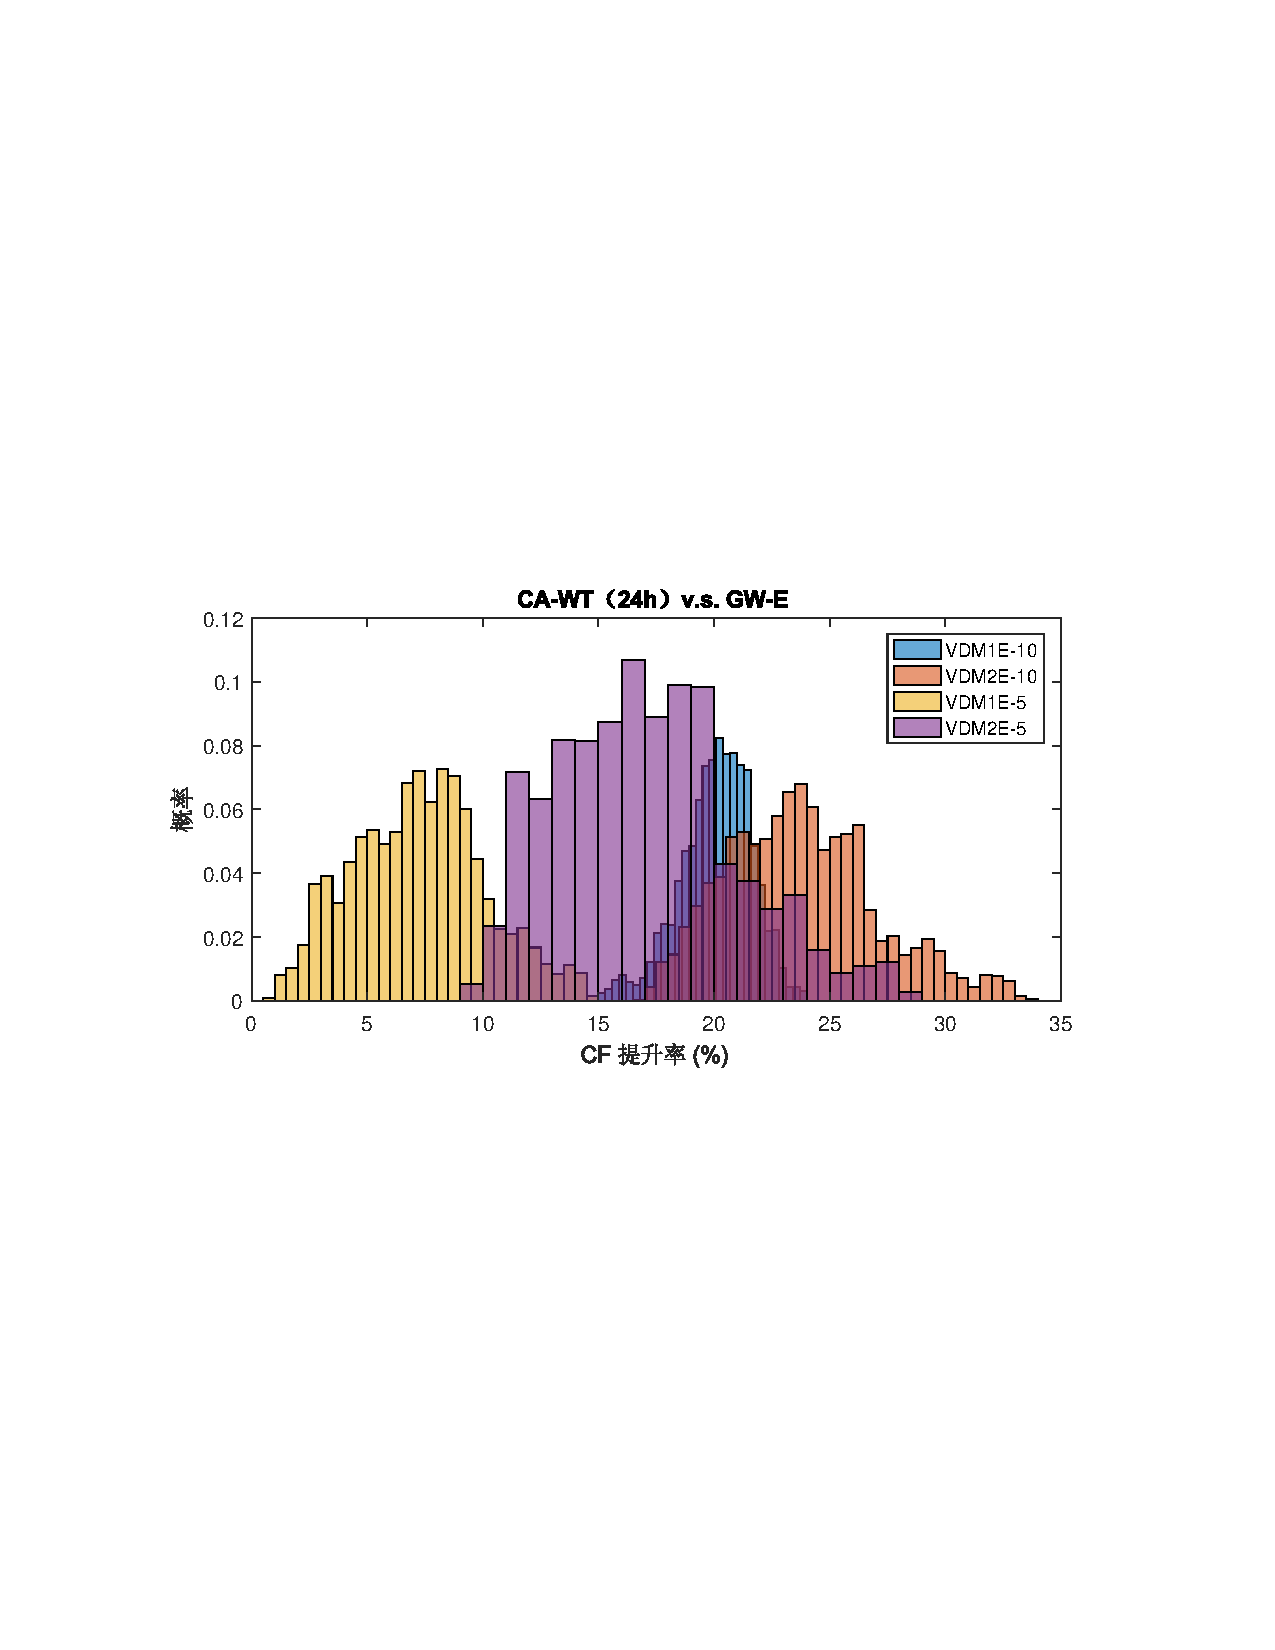
\includegraphics[scale=0.75]{figures/Chap5-CA-WT-24h-VS-GW-E.pdf}
  \caption{24h储能容量下叶片尺寸扩展的传统风机与灵活风机风机性能对比}
  \label{fig:CA-WT-24h-VS-GW-E}
\end{figure}

\begin{figure}[H] % use float package if you want it here
  \centering
  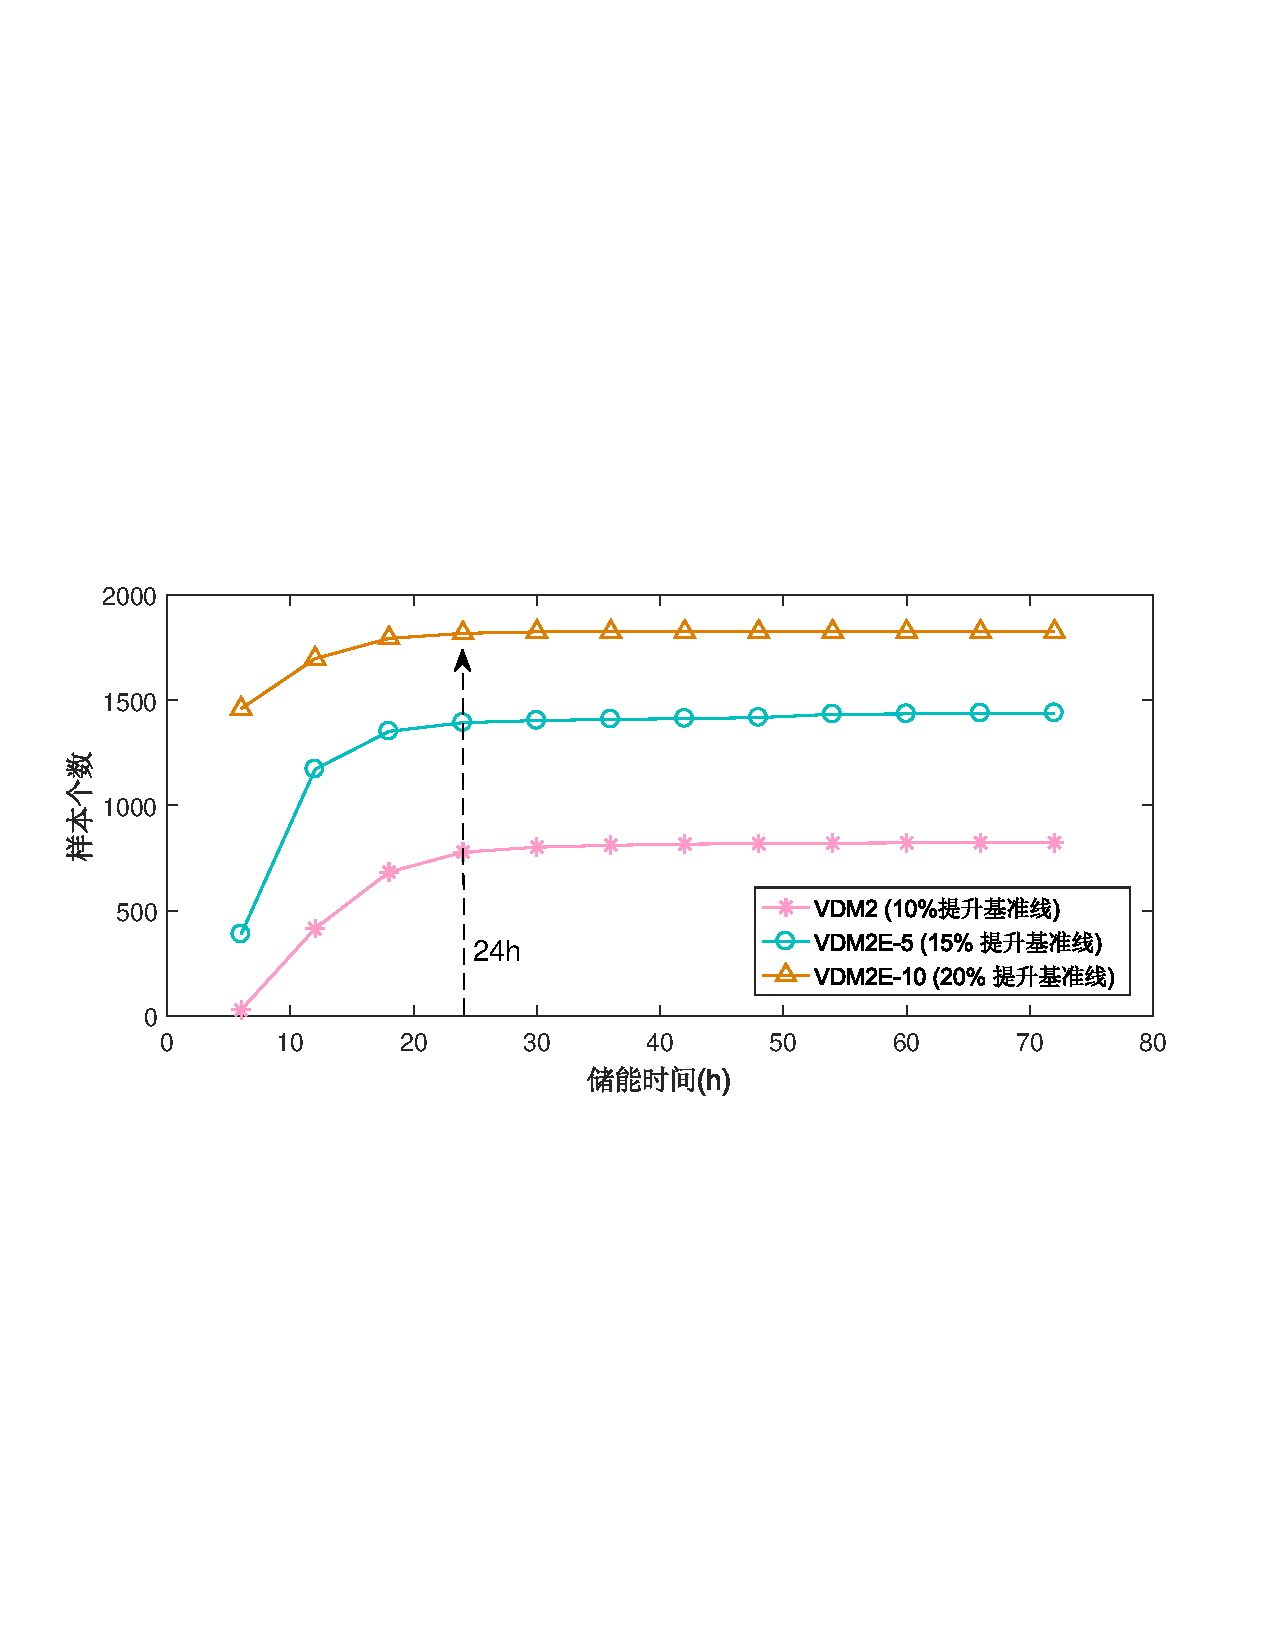
\includegraphics[scale=0.65]{figures/Chap5-CA-WT-Storage-Time-Sensitivity.pdf}
  \caption{灵活风机性能与储能容量的灵敏度}
  \label{fig:CA-WT-Storage-Time-Sensitivity}
\end{figure}

更为详细的灵敏度分析及相关数据,可参考本附录的(部分)开源代码,详见 https://github.com/AIRicky/Compressed-Air-Assisted-Wind-Turbine/tree/AIRicky-Sentivity.
